\section{Grafos}

\begin{frame}
	\begin{block}{Grafos}
		\begin{itemize}
			\item Um grafo é definido por $G = (V, E)$ onde: 
			\item V é um conjunto de vértices
			\item $E$ é um conjunto de arestas que relaciona, de alguma forma, os vértices
			\item $n = |V|$que é o número de vértices
			\item $m = |E|$ que é o número de arestas
		\end{itemize}
	\end{block}
\end{frame}

\begin{frame}
	\begin{block}{Grafos}
		Podemos ver um exemplo de grafo não dirigido:
		\begin{figure}[!htb]
			\centering	  				
			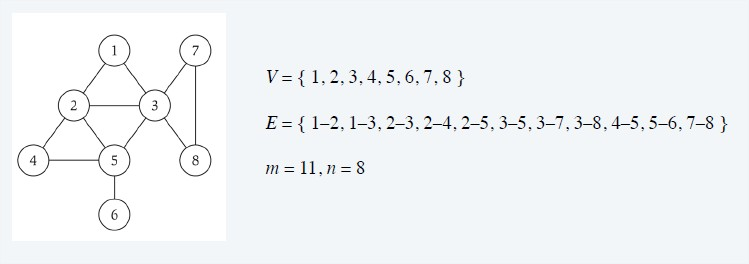
\includegraphics[height=3cm, width = 9cm]{./pic/grafoNaoDirigido.jpg}
			\caption{Exemplo de grafo não dirigido}
			\label{fig_pilha}
		\end{figure}
	\end{block}
\end{frame}

\begin{frame}
	\begin{block}{Grafos: Exemplo}
		Exemplo de uso:
		\begin{figure}[!htb]
			\centering	  				
			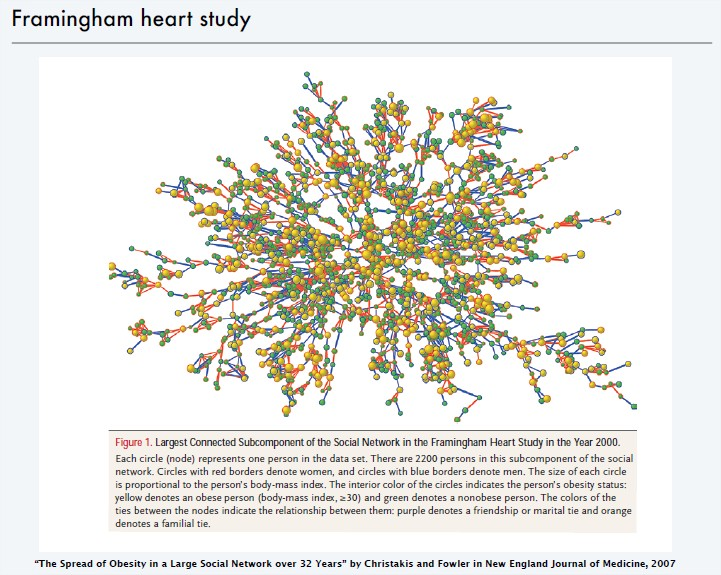
\includegraphics[height=7cm, width = 9cm]{./pic/exemploGrafo.jpg}
			\caption{Exemplo de grafo não dirigido}
			\label{fig_pilha}
		\end{figure}
	\end{block}
\end{frame}


\begin{frame}
	\begin{block}{Grafos}
		\begin{itemize}
			\item Qual a relação entre os vértices? Potencialmente qualquer uma, o que torna os grafos uma estrutura de dados com alto poder de modelar o mundo
			\item Diversos problemas científicos são modelados como grafo	
			\item Em games labirintos podem ser representados como grafos	
			\item Em computação problemas de caminhos mínimos podem ser representados por grafos
		\end{itemize}
	\end{block}
\end{frame}


\begin{frame}
	\begin{block}{Grafos: representação}
		Podemos representar grafos por matriz de adjacência. Onde cada aresta aparece repetida como na ilustração:
		\begin{figure}[!htb]
			\centering	  				
			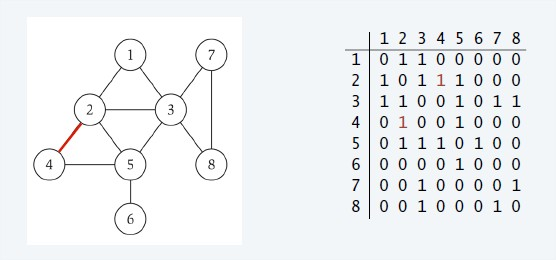
\includegraphics[height=4cm, width = 9cm]{./pic/matrizAdjacencia.jpg}
			\caption{Grafo representação por matriz de adjacência}
			\label{fig_pilha}
		\end{figure}
	\end{block}
\end{frame}

\begin{frame}
	\begin{block}{Grafos}
		\begin{itemize}
			\item Quais os pontos positivos e negativos sobre essa representação?	
			\item Vocês já tem o conhecimento sobre como implementar essa solução. Obs: é uma matriz..	
			\item Qual a complexidade de operações nessa estrutura de dados?
		\end{itemize}
	\end{block}
\end{frame}

\begin{frame}
	\begin{block}{Grafos: representação}
		Uma outra forma para representar grafos é usar uma lista de adjacências.  Como na ilustração:
		\begin{figure}[!htb]
			\centering	  				
			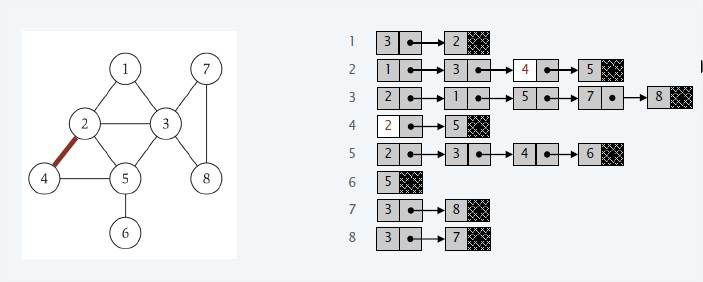
\includegraphics[height=4cm, width = 9cm]{./pic/listaAdjacencia.jpg}
			\caption{Grafo representação por lista de adjacências}
			\label{fig_pilha}
		\end{figure}
	\end{block}
\end{frame}

\begin{frame}
	\begin{block}{Grafos}
		\begin{itemize}
			\item Quais os pontos positivos e negativos sobre essa representação?	
			\item Vocês já tem o conhecimento sobre como implementar essa solução. Obs: é uma lista..	
			\item Qual a complexidade de operações nessa estrutura de dados?
		\end{itemize}
	\end{block}
\end{frame}

\begin{frame}
	\begin{block}{Grafos}
		\begin{itemize}
			\item Programar com os alunos em C\#
			\item Discutir no quadro a comparação com outras estruturas
		\end{itemize}
	\end{block}
\end{frame}

\begin{frame}
	\begin{block}{Grafos: definições}
		\begin{itemize}
			\item Caminho (Path) é uma sequência de nós conectados por arestas	
			\item Um grafo não dirigido é conectado se todos os pares de nós, dois a dois, tem uma aresta entre eles	
			\item Um ciclo em grafo não dirigido é um caminho onde o primeiro e último nó são iguais
		\end{itemize}
	\end{block}
\end{frame}

\begin{frame}
	\begin{block}{Grafos: definições}
		\begin{figure}[!htb]
			\centering	  				
			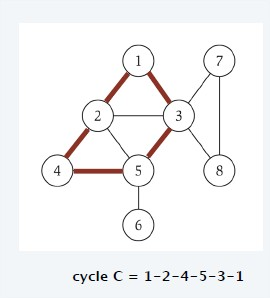
\includegraphics[height=4cm, width = 9cm]{./pic/ciclo.jpg}
			\caption{Grafo com ciclo}
			\label{fig_pilha}
		\end{figure}
	\end{block}
\end{frame}

\begin{frame}
	\begin{block}{Grafos: definições}
		Um grafo dirigido é considerado um árvore se ele não contém ciclos e estiver conectado.
		\begin{figure}[!htb]
			\centering	  
			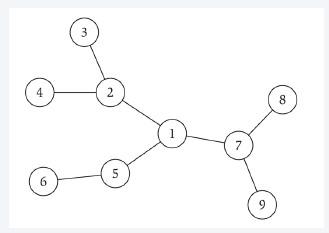
\includegraphics[height=4cm, width = 9cm]{./pic/arvoreGrafo.jpg}
			\caption{Grafo com ciclo}
			\label{fig_pilha}
		\end{figure}
	\end{block}
\end{frame}

\begin{frame}
	\begin{block}{Grafos: definições}
		Ao \emph{criar uma raiz} para o grafo, obtemos:
		\begin{figure}[!htb]
			\centering	  
			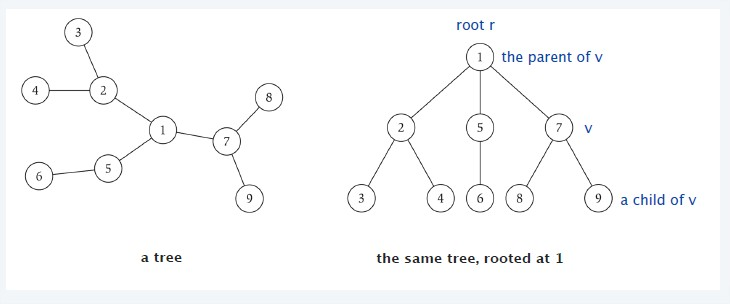
\includegraphics[height=4cm, width = 9cm]{./pic/grafoArvore2.jpg}
			\caption{Grafo com ciclo}
			\label{fig_pilha}
		\end{figure}
	\end{block}
\end{frame}

\begin{frame}
	\begin{block}{Grafos: problemas}
		\begin{itemize}
			\item Existe um caminho entre dois nós?
			\item Dados dois nós qual o caminho mínimo entre eles? Isso é uma forma de perguntar qual o menor caminho para atravessar um labirinto.	
			\item Alguma sugestão de como solucionar esse problema? De forma computacional
		\end{itemize}
	\end{block}
\end{frame}

\begin{frame}
	\begin{block}{Grafos: busca em largura}
		\begin{itemize}
			\item Dado um nó inicial, percorre o grafo todo de forma sistemática usando a seguinte estratégia:	
			\item Percorra os vizinhos do nó inicial, marque-os como visitados com um flag. Em seguida, percorra os vizinhos dos vizinhos $\ldots$ até que não tenham nós sem visitar.	
			\item Dado que grafos possuem ciclos, precisamos marcar os nós já visitados para evitar entrar em loop infinito.
		\end{itemize}
	\end{block}
\end{frame}


\begin{frame}
	\begin{block}{Grafos: busca em largura}
		\begin{figure}[!htb]
			\centering	  
			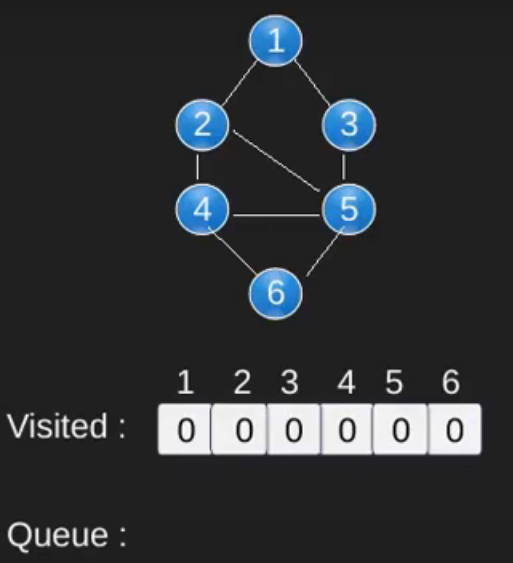
\includegraphics[height=4cm, width = 9cm]{./pic/bfs1.png}
			\caption{Grafo busca em largura}
		\end{figure}
	\end{block}
\end{frame}

\begin{frame}
	\begin{block}{Grafos: busca em largura}
		\begin{figure}[!htb]
			\centering	  
			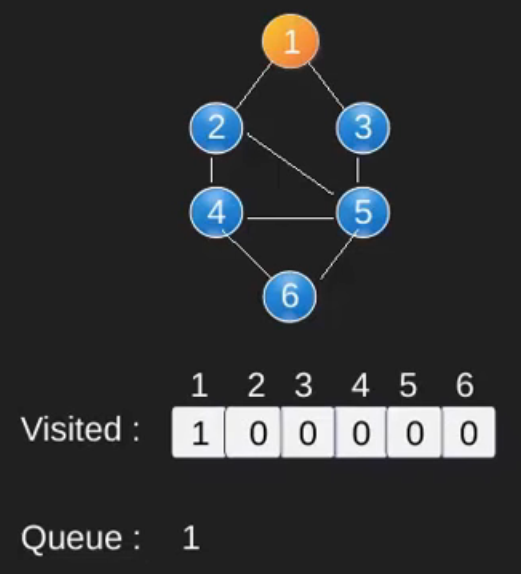
\includegraphics[height=4cm, width = 9cm]{./pic/bfs2.png}
			\caption{Grafo busca em largura}
		\end{figure}
	\end{block}
\end{frame}

\begin{frame}
	\begin{block}{Grafos: busca em largura}
		\begin{figure}[!htb]
			\centering	  
			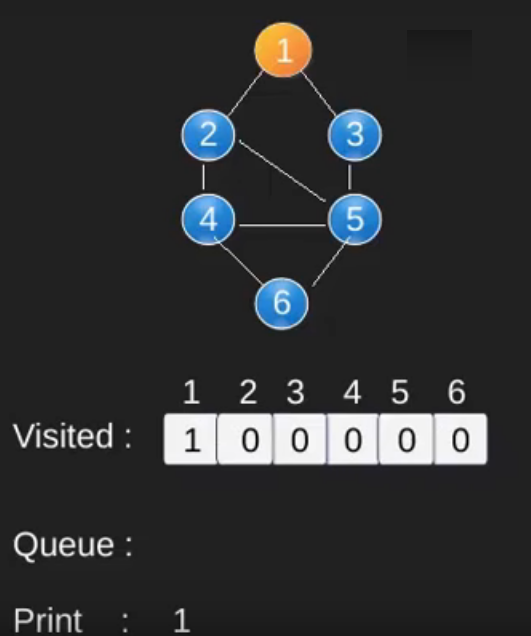
\includegraphics[height=4cm, width = 9cm]{./pic/bfs3.png}
			\caption{Grafo busca em largura}
		\end{figure}
	\end{block}
\end{frame}

\begin{frame}
	\begin{block}{Grafos: busca em largura}
		\begin{figure}[!htb]
			\centering	  
			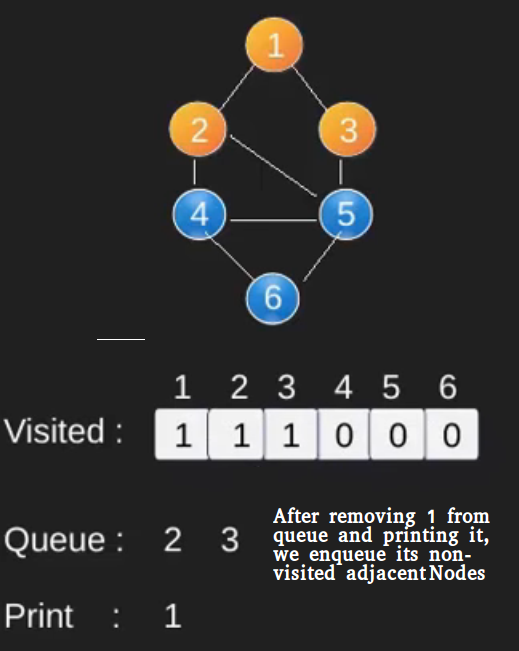
\includegraphics[height=4cm, width = 9cm]{./pic/bfs4.png}
			\caption{Grafo busca em largura}
		\end{figure}
	\end{block}
\end{frame}

\begin{frame}
	\begin{block}{Grafos: busca em largura}
		\begin{figure}[!htb]
			\centering	  
			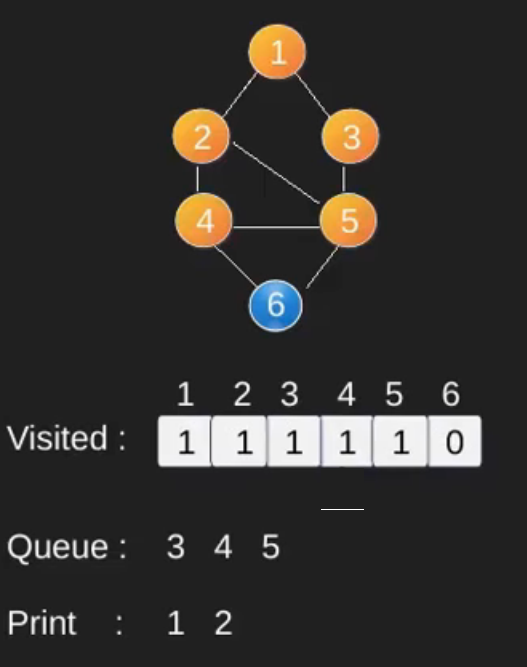
\includegraphics[height=4cm, width = 9cm]{./pic/bfs6.png}
			\caption{Grafo busca em largura}
		\end{figure}
	\end{block}
\end{frame}

\begin{frame}
	\begin{block}{Grafos: busca em largura}
		\begin{figure}[!htb]
			\centering	  
			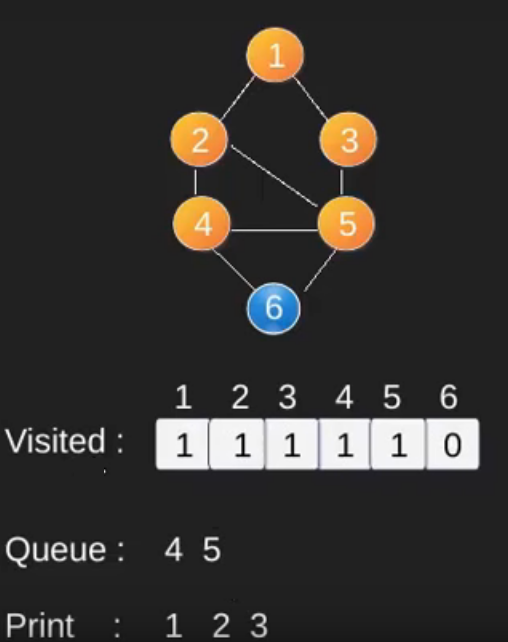
\includegraphics[height=4cm, width = 9cm]{./pic/bfs7.png}
			\caption{Grafo busca em largura}
		\end{figure}
	\end{block}
\end{frame}

\begin{frame}
	\begin{block}{Grafos: busca em largura}
		\begin{figure}[!htb]
			\centering	  
			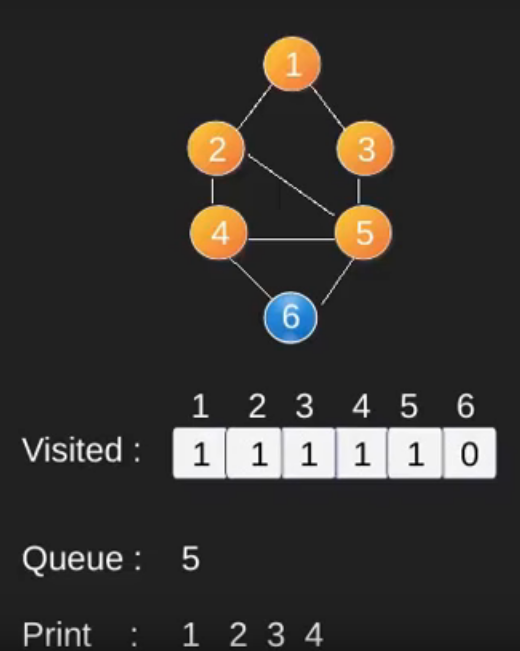
\includegraphics[height=4cm, width = 9cm]{./pic/bfs8.png}
			\caption{Grafo busca em largura}
		\end{figure}
	\end{block}
\end{frame}

\begin{frame}
	\begin{block}{Grafos: busca em largura}
		\begin{figure}[!htb]
			\centering	  
			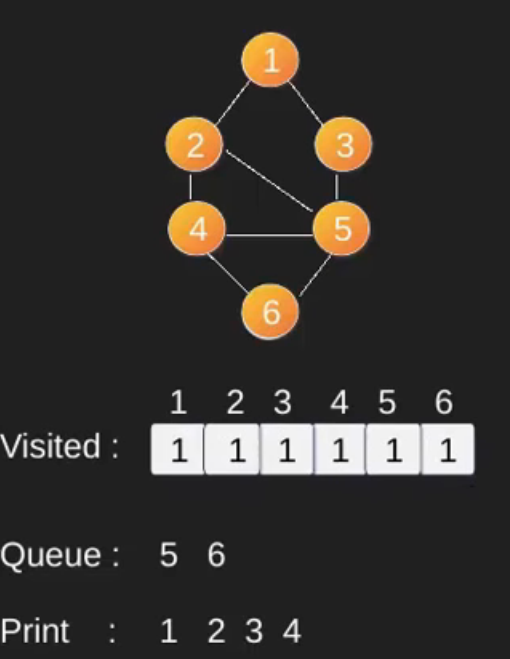
\includegraphics[height=4cm, width = 9cm]{./pic/bfs9.png}
			\caption{Grafo busca em largura}
		\end{figure}
	\end{block}
\end{frame}

\begin{frame}
	\begin{block}{Grafos: busca em largura}
		\begin{figure}[!htb]
			\centering	  
			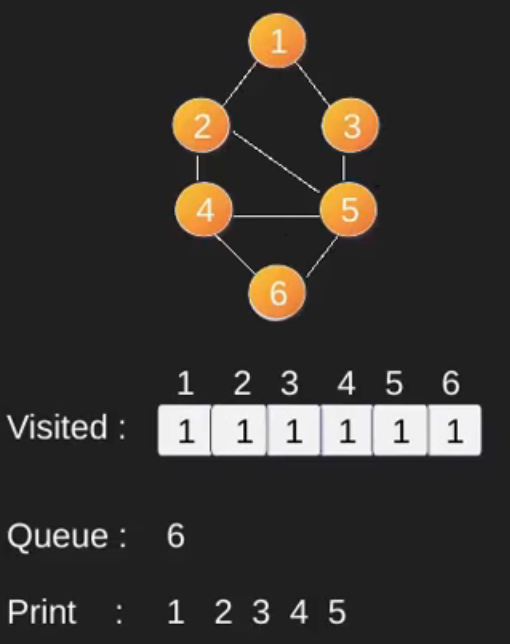
\includegraphics[height=4cm, width = 9cm]{./pic/bfs10.png}
			\caption{Grafo busca em largura}
		\end{figure}
	\end{block}
\end{frame}

\begin{frame}
	\begin{block}{Grafos: busca em largura}
		\begin{figure}[!htb]
			\centering	  
			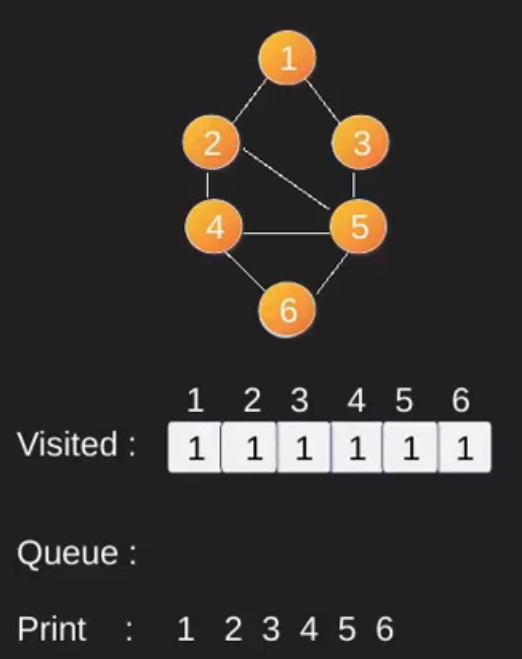
\includegraphics[height=4cm, width = 9cm]{./pic/bfs11.png}
			\caption{Grafo busca em largura}
		\end{figure}
	\end{block}
\end{frame}

\begin{frame}
	\begin{block}{Grafos}
		\begin{itemize}
			\item Programar com os alunos em C\#	
			\item Mostrar complexidade no quadro	
			\item Passar exercício para os alunos
		\end{itemize}
	\end{block}
\end{frame}

\begin{frame}
	\begin{block}{Grafos: busca em profundidade}
		\begin{itemize}
			\item Dado um nó inicial, percorre o grafo todo de forma sistemática usando a seguinte estratégia:
			\item Percorra um próximo vizinho do nó inicial, marque-o como visitado. Em seguida, percorra um vizinho daquele vizinho.
			\item A estratégia desse algoritmo é como a estratégia para percorrer uma árvore, o desafio adicional é considerar os ciclos possíveis dentro do grafo. Já tratados com a marcação de visitados.
		\end{itemize}
	\end{block}
\end{frame}


\begin{frame}
	\begin{block}{Grafos: busca em profundidade}
		\begin{figure}[!htb]
			\centering	  
			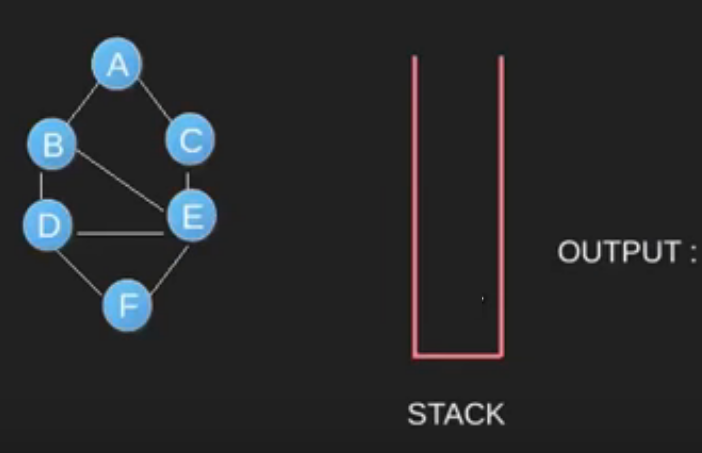
\includegraphics[height=4cm, width = 9cm]{./pic/dfs1.png}
			\caption{Grafo busca em profundidade}
		\end{figure}
	\end{block}
\end{frame}

\begin{frame}
	\begin{block}{Grafos: busca em profundidade}
		\begin{figure}[!htb]
			\centering	  
			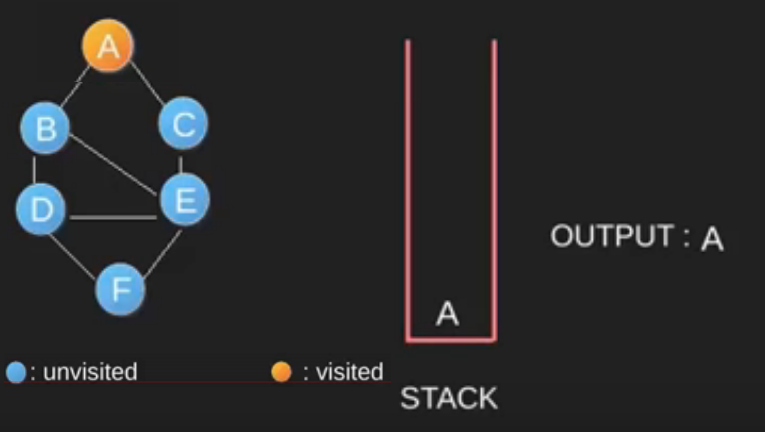
\includegraphics[height=4cm, width = 9cm]{./pic/dfs2.png}
			\caption{Grafo busca em profundidade}
		\end{figure}
	\end{block}
\end{frame}

\begin{frame}
	\begin{block}{Grafos: busca em profundidade}
		\begin{figure}[!htb]
			\centering	  
			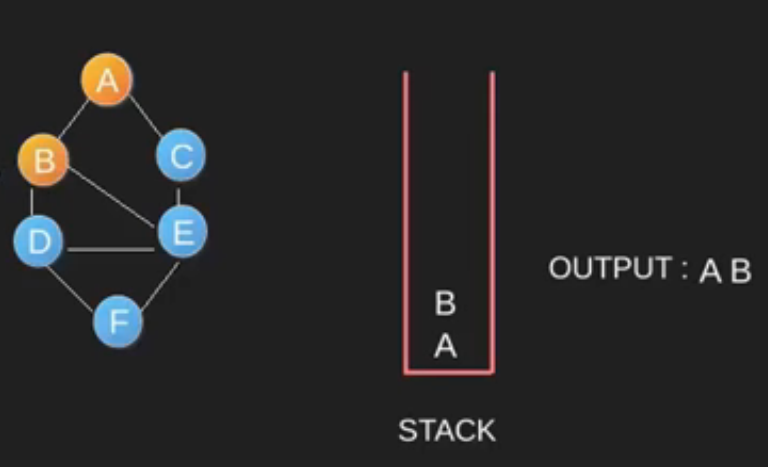
\includegraphics[height=4cm, width = 9cm]{./pic/dfs3.png}
			\caption{Grafo busca em profundidade}
		\end{figure}
	\end{block}
\end{frame}

\begin{frame}
	\begin{block}{Grafos: busca em profundidade}
		\begin{figure}[!htb]
			\centering	  
			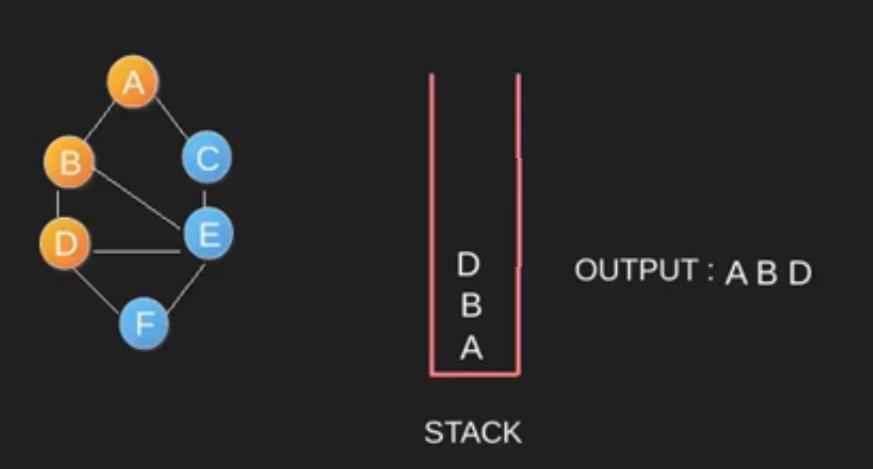
\includegraphics[height=4cm, width = 9cm]{./pic/dfs4.png}
			\caption{Grafo busca em profundidade}
		\end{figure}
	\end{block}
\end{frame}

\begin{frame}
	\begin{block}{Grafos: busca em profundidade}
		\begin{figure}[!htb]
			\centering	  
			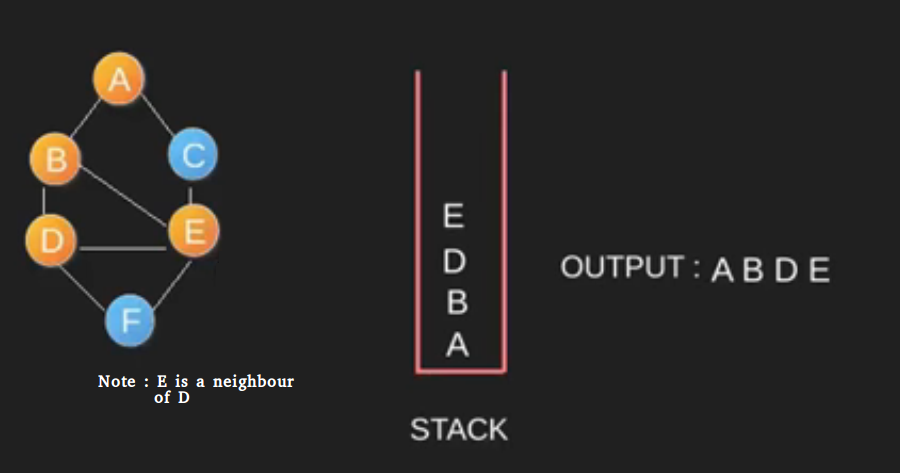
\includegraphics[height=4cm, width = 9cm]{./pic/dfs5.png}
			\caption{Grafo busca em profundidade}
		\end{figure}
	\end{block}
\end{frame}

\begin{frame}
	\begin{block}{Grafos: busca em profundidade}
		\begin{figure}[!htb]
			\centering	  
			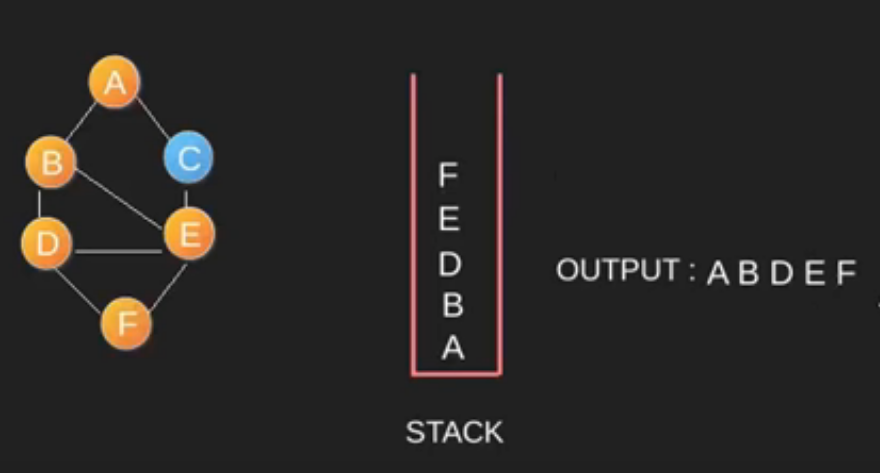
\includegraphics[height=4cm, width = 9cm]{./pic/dfs6.png}
			\caption{Grafo busca em profundidade}
		\end{figure}
	\end{block}
\end{frame}

\begin{frame}
	\begin{block}{Grafos: busca em profundidade}
		\begin{figure}[!htb]
			\centering	  
			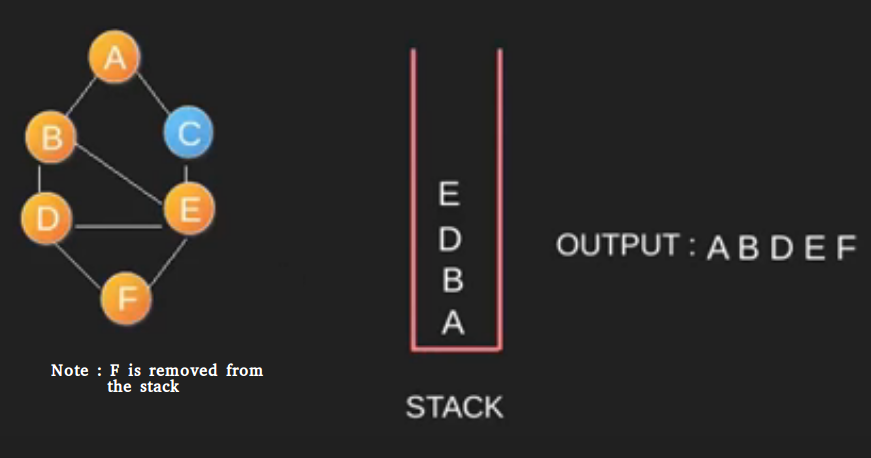
\includegraphics[height=4cm, width = 9cm]{./pic/dfs7.png}
			\caption{Grafo busca em profundidade}
		\end{figure}
	\end{block}
\end{frame}

\begin{frame}
	\begin{block}{Grafos: busca em profundidade}
		\begin{figure}[!htb]
			\centering	  
			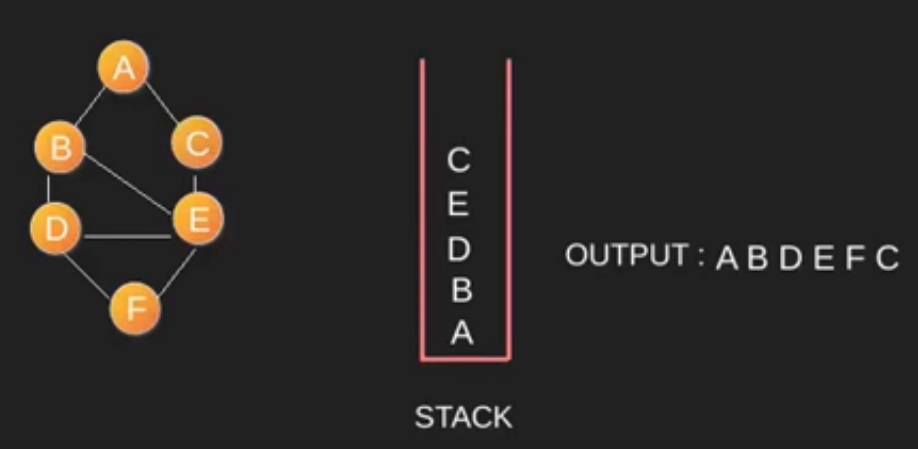
\includegraphics[height=4cm, width = 9cm]{./pic/dfs8.png}
			\caption{Grafo busca em profundidade}
		\end{figure}
	\end{block}
\end{frame}

\begin{frame}
	\begin{block}{Grafos: busca em profundidade}
		\begin{figure}[!htb]
			\centering	  
			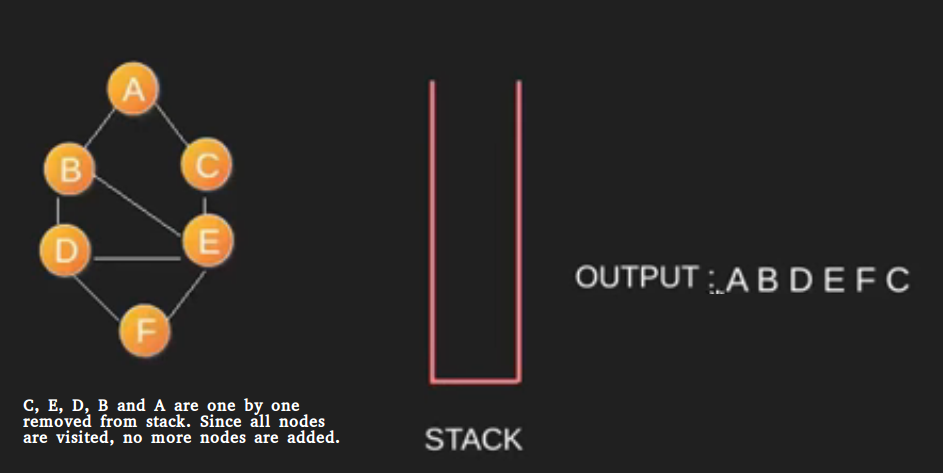
\includegraphics[height=4cm, width = 9cm]{./pic/dfs9.png}
			\caption{Grafo busca em profundidade}
		\end{figure}
	\end{block}
\end{frame}

\begin{frame}
	\begin{block}{Grafos}
		\begin{itemize}
			\item Programar com os alunos em C\#	
			\item Mostrar complexidade no quadro	
			\item Passar exercício para os alunos
		\end{itemize}
	\end{block}
\end{frame}

\begin{frame}
	\begin{block}{Grafos: mais definições}
		\begin{figure}[!htb]
			\centering	  
			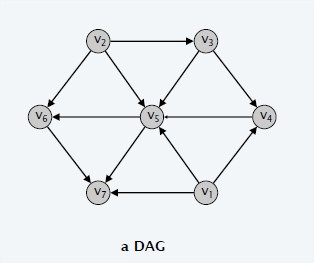
\includegraphics[height=4cm, width = 9cm]{./pic/DAGSemCiclo.jpg}
			\caption{Grafos mais definições}
		\end{figure}
	\end{block}
\end{frame}

\begin{frame}
	\begin{block}{Grafos: mais definições}
		O grafo abaixo apresenta ciclos? Se sim, quais? 
		\begin{figure}[!htb]
			\centering	  
			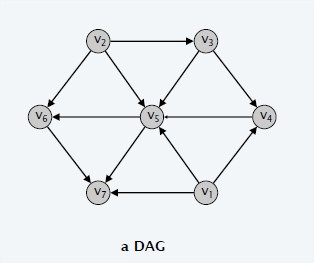
\includegraphics[height=4cm, width = 9cm]{./pic/DAGSemCiclo.jpg}
			\caption{Grafos mais definições}
		\end{figure}
	\end{block}
\end{frame}

\begin{frame}
	\begin{block}{Grafos: mais definições}
		Algoritmos de grafo não dirigido se aplicam aqui?
		\begin{figure}[!htb]
			\centering	  
			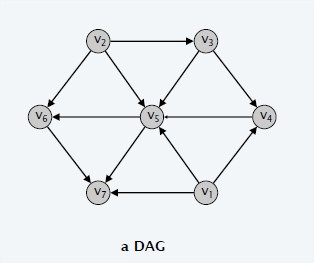
\includegraphics[height=4cm, width = 9cm]{./pic/DAGSemCiclo.jpg}
			\caption{Grafos mais definições}
		\end{figure}
	\end{block}
\end{frame}

\begin{frame}
	\begin{block}{Grafos}
		\begin{itemize}
			\item Dado um grafo e um nó “fonte”, encontre o caminho mínimo para todos os outros nós desse grafo.
			\item Existe o algoritmo de Dijkstra para resolver esse problema com os seguintes passos:
			\item Cria uma árvore de caminho mínimo, atribuí um valor de distância infinito para cada nó menos o “fonte” que terá distância zero
			\item Enquanto a árvore de caminho mínimo não contiver todos os nós:
			\item Pegue um vértice fora da árvore
			\item Adicione na árvore
			\item Atualize todos os nós vizinhos desse novo vértice.
		\end{itemize}
	\end{block}
\end{frame}

\begin{frame}
	\begin{block}{Grafos: Caminhos mínimos}
		\begin{figure}[!htb]
			\centering	  
			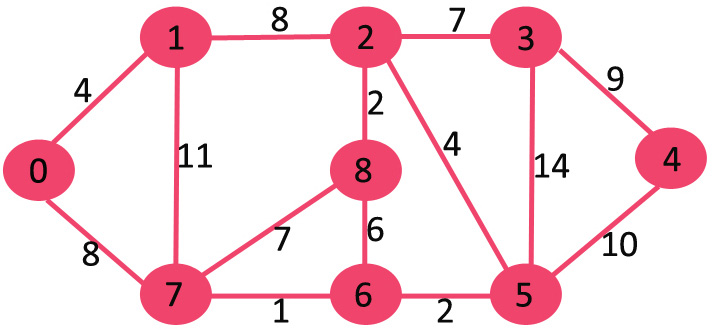
\includegraphics[height=4cm, width = 9cm]{./pic/Fig-11.jpg}
			\caption{Grafos caminhos mínimos}
		\end{figure}
	\end{block}
\end{frame}

\begin{frame}
	\begin{block}{Grafos: Dijsktra}
		Inicializa o vetor de distâncias para cada vértice com infinito menos o vértice escolhido como \emph{fonte}. Em seguida, actualize a distância dos vertices adjacentes
		\begin{figure}[!htb]
			\centering	  
			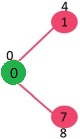
\includegraphics[height=4cm, width = 9cm]{./pic/MST1.jpg}
			\caption{Grafos Dijsktra}
		\end{figure}
	\end{block}
\end{frame}

\begin{frame}
	\begin{block}{Grafos: Dijsktra}
		Do conjunto de vertices não incluídos pegue aquele com menor distância e inclua ele na árvore de caminho mínimo. Atualize o peso dos nós adjacentes.
		\begin{figure}[!htb]
			\centering	  
			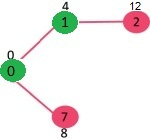
\includegraphics[height=4cm, width = 9cm]{./pic/DIJ2.jpg}
			\caption{Grafos Dijsktra}
		\end{figure}
	\end{block}
\end{frame}

\begin{frame}
	\begin{block}{Grafos: Dijsktra}
		Do conjunto de vertices não incluídos pegue aquele com menor distância e inclua ele na árvore de caminho mínimo. Atualize o peso dos nós adjacentes.
		\begin{figure}[!htb]
			\centering	  
			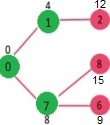
\includegraphics[height=4cm, width = 9cm]{./pic/DIJ3.jpg}
			\caption{Grafos Dijsktra}
		\end{figure}
	\end{block}
\end{frame}

\begin{frame}
	\begin{block}{Grafos: Dijsktra}
		Do conjunto de vertices não incluídos pegue aquele com menor distância e inclua ele na árvore de caminho mínimo. Atualize o peso dos nós adjacentes.
		\begin{figure}[!htb]
			\centering	  
			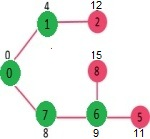
\includegraphics[height=4cm, width = 9cm]{./pic/DIJ4.jpg}
			\caption{Grafos Dijsktra}
		\end{figure}
	\end{block}
\end{frame}

\begin{frame}
	\begin{block}{Grafos: Dijsktra}
		Repita esse processo até que todos os nós sejam incluídos
		\begin{figure}[!htb]
			\centering	  
			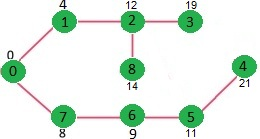
\includegraphics[height=4cm, width = 9cm]{./pic/DIJ5.jpg}
			\caption{Grafos Dijsktra}
		\end{figure}
	\end{block}
\end{frame}

\begin{frame}
	\begin{block}{Grafos: Dijsktra x Prim}
		\begin{itemize}
			\item Algumas pessoas confundem os algoritmos de Dijkstra e Prim (não dirigidos). Vale ressaltar que a árvore geradora minima (PRIM) garante que todos os nós sejam conectados com o custo mínimo para conectar todos os nós.
			\item A árvore de caminho mínimo garante o caminho mínimo de todos os nós para um determinado nó denominado: \emph{fonte}.
			\item O algoritmo de Dijkstra tem problemas em arestas com peso negative, o algoritmo de Prim lida com eles. O algoritmo de Prim lida com apenas grafos não dirigidos.
		\end{itemize}
	\end{block}
\end{frame}

\begin{frame}
	\begin{block}{Grafos}
		\begin{itemize}
			\item Programar com os alunos em C\#	
			\item Mostrar complexidade no quadro	
			\item Passar exercício para os alunos
		\end{itemize}
	\end{block}
\end{frame}


